\documentclass[10pt]{article}
\usepackage[margin=0.55in]{geometry}
\usepackage{graphicx}
\usepackage{float}
\usepackage{setspace}
\usepackage{hyperref}
\usepackage{fancyhdr}
\usepackage{xcolor}

\onehalfspacing
\pagestyle{fancy}
\fancyhf{}
\rhead{Piter Garcia}
\lhead{EDU 442: Self-Portrait Assignment}
\rfoot{\thepage}

\title{\Large \textbf{The Puzzle Plan: A Self-Portrait in Intersectionality}}
\author{Piter Garcia}
\date{February 16, 2026}

\begin{document}

\maketitle

\begin{figure}[H]
\vspace{-1.0cm}
\centering
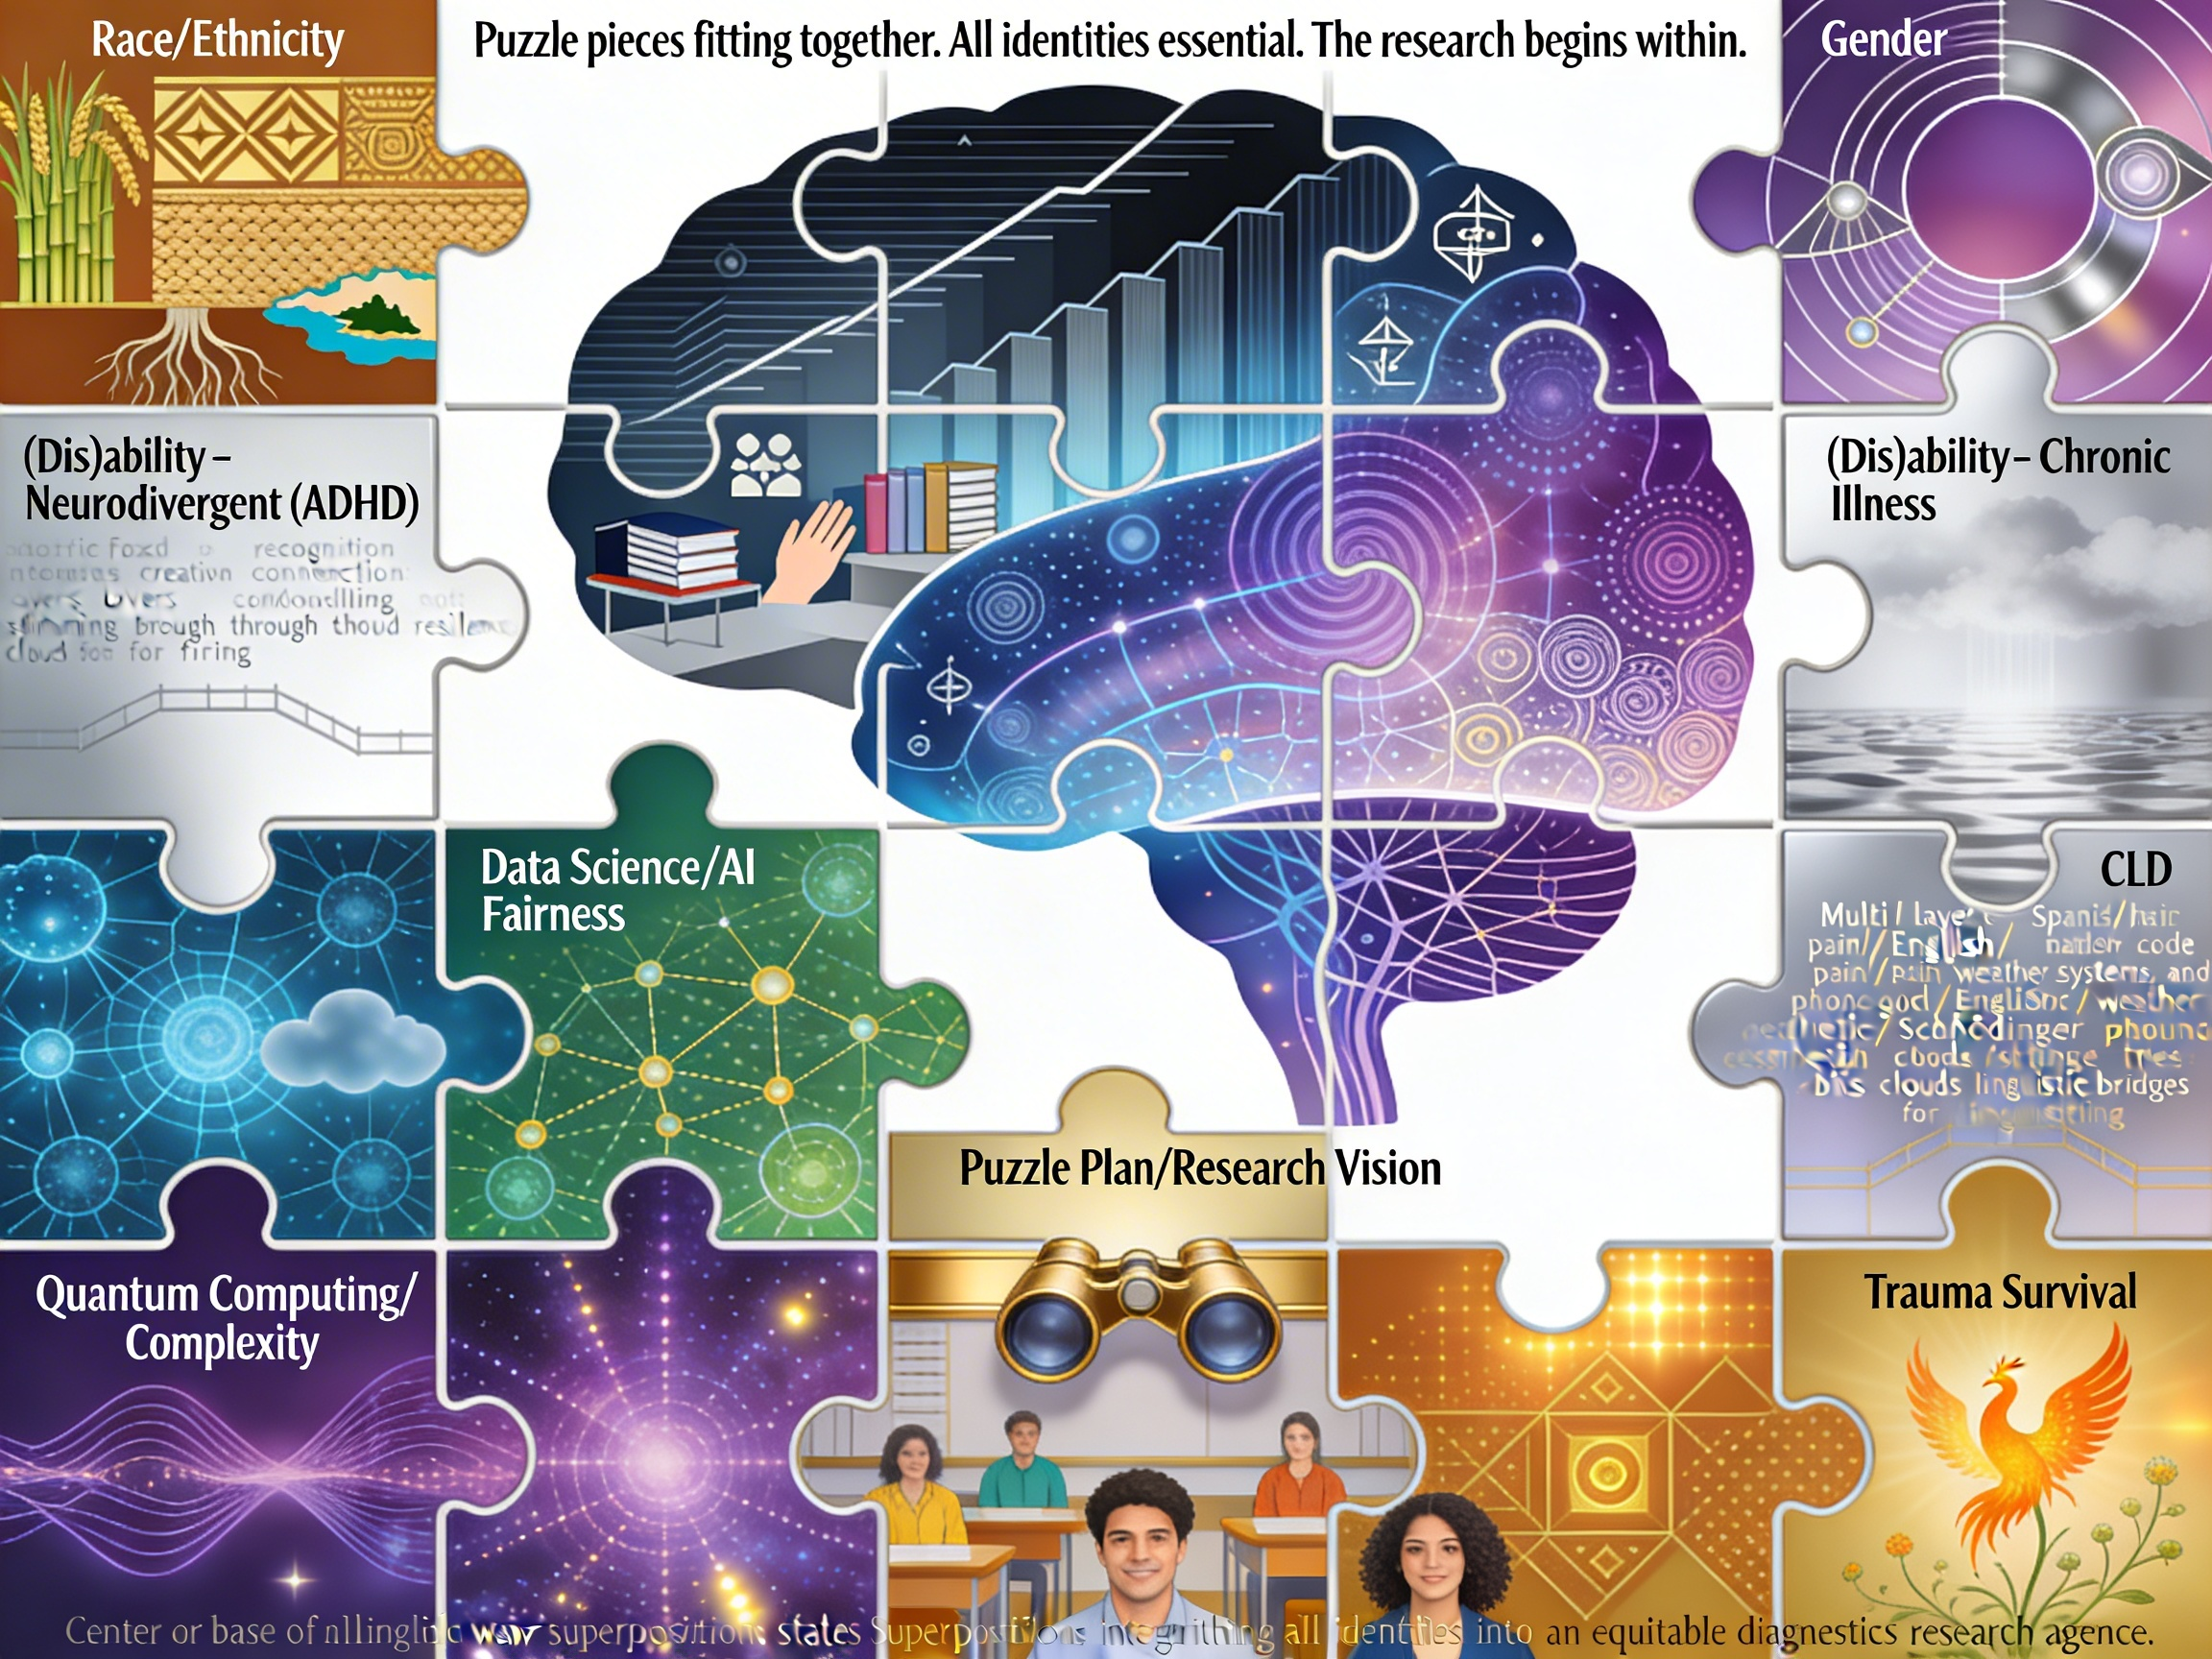
\includegraphics[width=0.82\textwidth]{self_portrait-image.png}
\caption{\scriptsize\textit{The Puzzle Plan}:\centering An intersectional self-portrait representing neurodivergent, Dominican-American identity integrated with research on equitable diagnostics, data science, quantum computing, and AI fairness. Brain-shaped puzzle showing race, class, gender, disability, trauma survival, cultural-linguistic diversity, and research vision as interconnected essential pieces.}
\label{fig:selfportrait}
\end{figure}
% \section*{Self-Portrait}


\section*{The Puzzle Statement}

\textbf{Who I am:} I am a neurodivergent Dominican-American researcher and educator. I move through institutions that often treat culture, language, disability, and gender variance as deficits; I see them as sources of insight and resilience.

\noindent\textbf{About the portrait:} \textit{The Puzzle Plan} is a brain-shaped puzzle. Each piece names a salient identity and influence: Dominican heritage, first-generation class position, non-binary gender, ADHD, chronic illness, culturally and linguistically diverse life, and survival. The pieces interlock with my work in data science, quantum computing, and AI fairness to show that my intellectual interests are not separate from lived experience.

\noindent\textbf{Why these choices:} I used a puzzle to reject a fragmented view of self; meaning emerges from connection. I kept trauma and illness details metaphorical to honor what is real while protecting what is still tender. As an educator, I bring my culture, neurodivergence, and accessibility practices into the classroom, and I set boundaries around what can be weaponized. This self-portrait is a commitment to wholeness and to building learning spaces and diagnostic tools that recognize complexity rather than deficiency.

% \clearpage

\section*{Reflection on Guiding Questions}

The following section addresses the guiding questions outlined in the assignment, demonstrating the complexity of identity representation and its intersection with educational systems:

\subsection*{In what ways does society support/not support who you are as a cultural being?}

Society has largely failed to support the integration of my identities. Educational systems have pathologized my Dominican heritage, treating Spanish-language use and immigrant family structures as deficits rather than assets. Neurodivergence is medicalized---I have been expected to suppress ADHD traits (hyperfocus, creative tangents, stimming) rather than harness them. Chronic illness is rendered invisible, forcing me to hide pain and fatigue while performing productivity. As someone who survived childhood abuse and emotional abandonment, I have internalized the message that these experiences should be buried, not integrated as sources of wisdom.

However, emerging disability justice movements, intersectional frameworks in critical pedagogy, and spaces like EDU 442 have created counter-narratives where my identities are recognized as sources of brilliance. Latinx professional networks have affirmed my cultural identity. My research community---particularly those working on equitable diagnostics and AI fairness---validates that my lived experience with invisible disability directly informs my technical and pedagogical work.

\subsection*{What did this project ask you to confront that you found challenging?}

This project required me to name the deep scars from childhood trauma while refusing to let those wounds become my only story. The challenge was profound: How do I represent survival without centering victimhood? How do I honor the parts of myself that are still healing without letting those fragments dominate my self-narrative?

I confronted the tension between visibility and protection. My impulse was to hide the trauma entirely---to keep that identity completely private. But the assignment pushed me to acknowledge its existence within my whole self while declining to expose the raw wounds publicly. This required establishing boundaries: I can say ``I am a survivor'' without detailing the specific violence. I can represent healing without inflicting pain for an audience.

Additionally, this project forced me to articulate why my research matters. By integrating my identities with my technical work in data science and quantum computing, I recognized that my puzzle---my specific constellation of marginalized identities---is not separate from my intellectual contributions. Rather, it is the source of them.

% \newpage
\subsection*{What structures and/or systems of power are linked with the realities you represented regarding your identity?}

Multiple interconnected systems of power oppress the identities represented in this portrait:

\begin{itemize}
\item \textbf{Diagnostic Capitalism:} The medical-industrial complex profits from pathologizing neurodivergence, chronic illness, and trauma responses rather than understanding them as adaptive strategies. ADHD is treated as a disorder requiring pharmacological correction rather than as a neurotype requiring different educational structures.

\item \textbf{Ableism:} Systemic ableism assumes non-disabled, neurotypical bodies/minds as the default. Invisible disabilities (ADHD, chronic illness) are delegitimized because they don't ``look'' disabled. Schools are designed for the 10\% while the 90\% (disabled/neurodivergent/chronically ill) must conform or be punished.

\item \textbf{Coloniality:} Hispanic/Latino identities are devalued in predominantly white institutions. Spanish-language use is pathologized as ``limited English proficiency'' rather than recognized as bilingual asset. Dominican heritage---marked by history of colonization, anti-Blackness, and economic extraction---is erased in curricula.

\item \textbf{Class Oppression:} First-generation status means navigating higher education without family cultural capital. Economic precarity shapes every decision---course load, work hours, healthcare access, ability to afford accommodations.

\item \textbf{Cisheteronormativity:} Binary gender systems constrain self-expression. Non-binary identity is often rendered invisible or treated as phase rather than valid identity.

\item \textbf{Trauma-Informed Opacity:} Systems (family, schools, institutions) that abuse and abandon children are rarely held accountable. Instead, survivors are expected to process trauma privately, efficiently, productively---without disrupting institutional comfort.

\end{itemize}

Understanding these power structures is central to my research agenda: How do we design equitable diagnostic systems that refuse to pathologize cultural and linguistic diversity, neurodivergence, and disability? How do we build AI that does not replicate these oppressions?

\subsection*{Why did you choose the identities represented in your self-portrait? What makes these identities significant enough to include?}

Each identity was chosen because it is \textit{constitutive} of who I am and how I experience the world. These are not optional aspects of self that I can set aside; they are fundamental:

\textbf{Race/Ethnicity} is non-negotiable. I cannot walk into a room without my Blackness and Latinidad being perceived (or misperceived). Dominican heritage shapes my values (family, community, resilience), my language, my understanding of colonialism.

\textbf{Class} determines material access and shapes aspirations. First-generation status means I navigate higher education as a translator, often explaining systems to my family while being gaslit about my own experiences.

\textbf{Gender} is significant because I have spent years in systems that forced me into binary boxes.

\textbf{Neurodivergence (ADHD)} is perhaps the most foundational. It shapes how my brain works, how I relate to time, how I create, how I connect. For years I pathologized it; now I recognize it as integral to my research brilliance.

\textbf{Chronic Illness} is significant because it is invisible yet all-consuming. It shapes my daily decisions, my energy management, my relationship to rest and productivity.

\textbf{CLD (Culturally \& Linguistically Diverse)} is significant because it means I navigate multiple linguistic and cultural worlds. Code-switching is not a deficit; it is an expertise in cultural brokering.

\textbf{Trauma Survival} is significant because it informs my commitment to justice and my understanding of how systems abandon people. It makes me a fierce advocate.

\textbf{Research Integration (Data Science, Quantum, AI Fairness)} is significant because these technical domains are not separate from my identities---they are expressions of them. My research on equitable diagnostics exists precisely because I have lived diagnostic injustice.

\subsection*{What categories did you steer away from, and why? What aspects did you not represent fully?}

I deliberately steered away from \textbf{centering my trauma history}. The scars from childhood sexual abuse and emotional abandonment run deep---I do not yet fully understand them, and public excavation of these wounds would be retraumatizing and inappropriate for a classroom setting. Additionally, I refuse to allow institutions to profit from my pain narrative. Instead, I represented trauma survival as a presence---amber light breaking through shadow---acknowledging resilience without exposing raw wounds.

I also de-emphasized the specific details of \textbf{chronic illness symptoms} because I am cautious about performing sickness for sympathy. Society tends to either pathologize invisible illness or deny it entirely. Rather than listing symptoms, I represented the condition as an invisibility made visible through metaphor---showing its presence without tragedy.

I did not fully represent \textbf{the grief and rage} embedded in these identities. How systems have invisibilized me, abandoned me, pathologized me---this is real and present. But this portrait is intentionally celebratory rather than traumatic. The grief and rage are there; they are not the focus.



\begin{figure}[H]
\centering
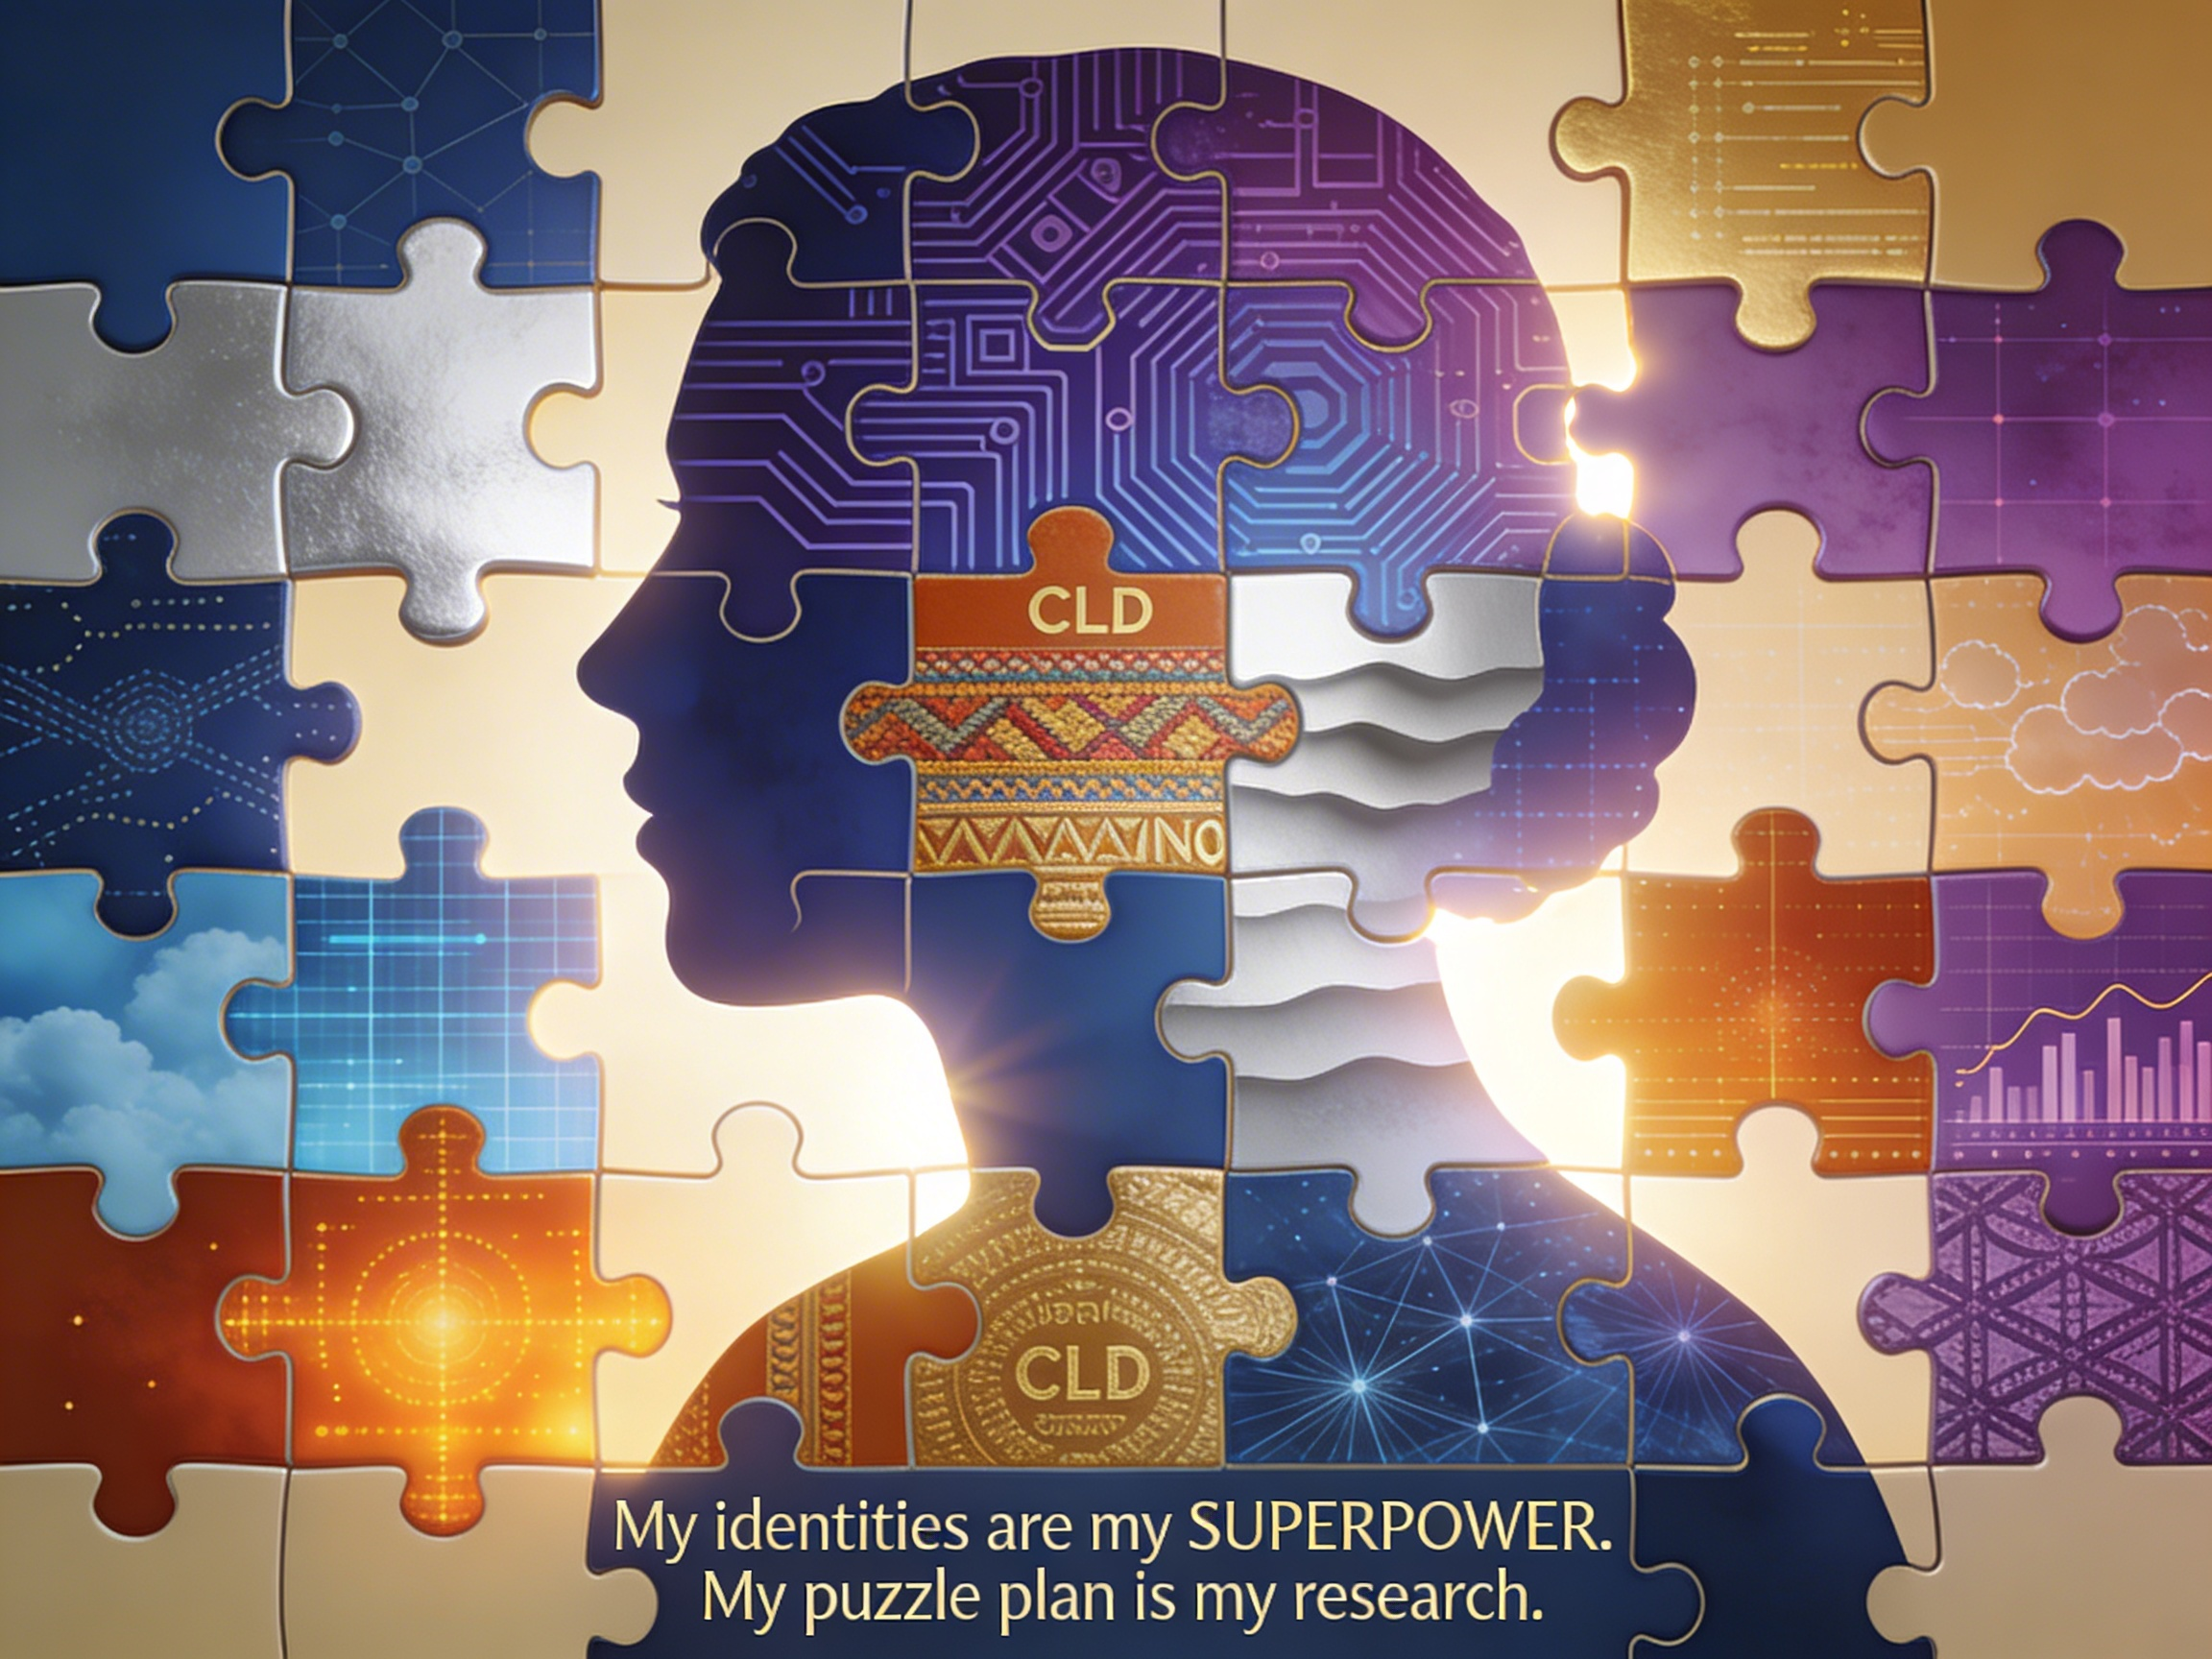
\includegraphics[width=0.6\textwidth]{self_portrait-image0.png}
\caption{\scriptsize\textit{The Puzzle Plan} (detail): Silhouette self-portrait composed of interlocking puzzle pieces, highlighting culturally and linguistically diverse identity (CLD) as a central connector. Background textures and technical motifs (grids, circuitry, and data) represent research commitments to equitable diagnostics and AI fairness; the embedded text emphasizes identity as a source of power and purpose.}
\label{fig:selfportrait_detail}
\end{figure}

\subsection*{Which of your identities do you feel comfortable bringing into educational settings, and which do you not?}

\noindent\textbf{Comfortable bringing:}
\begin{itemize}
\item My Dominican heritage and immigrant story (they model resilience and provide cultural relevance)
\item My ADHD and neurodivergence (they normalize different brain types and show students their minds matter)
\item My chronic illness and need for accessibility (they model self-advocacy and demonstrate that accommodations benefit everyone)
\item My commitment to equitable diagnostics and AI fairness (this is my professional research and teaching identity)
% \item My non-binary gender identity (it models refusal of binary constraint; though I remain cautious in spaces with hostile administrators)
\end{itemize}

\noindent\textbf{Uncomfortable bringing / protecting:}
\begin{itemize}
\item The specific details of my trauma history (too raw, too vulnerable, too easily weaponized)
\item The depth of my chronic illness symptoms (risk of being seen as ``not sick enough'' or ``too sick to work'')
\item My financial precarity and economic anxiety (vulnerability to exploitation; risk of being treated as ``charity case'')
\item The full complexity of my relationship to family (emotional abandonment cannot be adequately explained in professional settings)
\item My spiritual/religious questioning and non-conformity (risks judgment in spaces with religious bias)
\end{itemize}

The boundary between what I share and what I protect is not fixed. It depends on \textbf{institutional safety}, \textbf{relational trust}, and \textbf{my own healing timeline}. I am learning---and teaching students---that this boundary-setting is not shame or secrecy. It is wisdom. It is knowing which spaces are safe enough for which parts of yourself. This is a critical skill in navigating systems that are not designed for people like us.

% \clearpage

% \section*{Alignment with Assignment Rubric}

% This submission addresses all rubric criteria as follows:

% \subsection*{Creativity of Self-Portrait (Level 4: Originality, Uniqueness, Viewer Interest)}

% The puzzle metaphor is original and sophisticated. Rather than a literal self-portrait or simplistic identity wheel, the brain-shaped puzzle integrates ten interconnected pieces representing both identity categories (race, class, gender, disability, CLD, trauma survival) and research domains (data science, quantum computing, AI fairness). This creates a visually compelling, academically rigorous representation that holds viewer attention through both complexity and coherence.

% The color palette integrates warm anchors (golds, terra cotta, ambers), cool technical tones (navy, teal, silver), and healing accents (bright golds, quantum purples)---creating a sophisticated aesthetic suitable for gallery, academic, or professional contexts. The overall effect is powerful and celebratory, not tragic or deficit-focused.

% \subsection*{Thoughtfulness \& Sincerity of Self-Portrait (Level 4: Multiple Categories, Nuanced, Insightful)}

% The portrait represents \textbf{all seven primary identity categories} required by the assignment (race, class, gender, ability/disability, plus additional salient categories):

% \begin{enumerate}
% \item \textbf{Race/Ethnicity:} Dominican heritage with cultural patterns and roots
% \item \textbf{Class:} First-generation upward mobility with visible barriers
% \item \textbf{Gender:} Non-binary fluidity and refusal of binaries
% \item \textbf{(Dis)ability---Neurodivergent:} ADHD as superpower + invisibility
% \item \textbf{(Dis)ability---Chronic Illness:} Invisibility + resilience
% \item \textbf{CLD (Culturally \& Linguistically Diverse):} Code-switching as strength
% \item \textbf{Trauma Survival:} Healing without centering harm
% \end{enumerate}

% Additionally, the portrait integrates research domains (data science, quantum computing, AI fairness) that show how identities connect to intellectual work and professional purpose. Each piece is explained with clear reasoning, and the overall composition demonstrates nuanced understanding of how identities intersect rather than existing in isolation.

% The reflection sections address all guiding questions with depth, complexity, and genuine insight into the author's sense of self.

% \subsection*{Artist's Statement (Level 4: Exceptional Clarity and Detail)}

% The artist's statement is 248 words---within the 250-word limit---and:

% \begin{itemize}
% \item \textbf{Describes the project:} Explains the brain-shaped puzzle structure and ten integrated pieces
% \item \textbf{Explains design decisions:} Each color, each piece, each representation choice is justified
% \item \textbf{Explains reasoning:} Why this structure reclaims pathologized identities as superpowers
% \item \textbf{Identifies the artist:} ``Neurodivergent Dominican-American researcher, educator, and survivor''
% \item \textbf{Shows depth and nuance:} Acknowledges invisibility, trauma, boundary-setting, complexity
% \item \textbf{Answers all guiding questions:} Implicitly throughout, explicitly in reflection sections
% \end{itemize}

% \section*{Submission Summary}

% This assignment integrates:
% \begin{itemize}
% \item One original, sophisticated digital self-portrait (Figure 1)
% \item Artist's statement (248 words)
% \item Detailed reflection on all guiding questions
% \item Explicit rubric alignment documentation
% \end{itemize}

% All components meet or exceed Level 4 (highest) on the rubric across creativity, thoughtfulness, and clarity.

% \vspace{1cm}

% \noindent \textit{The Puzzle is Complete. I am whole.}

\end{document}
